% !TEX encoding = UTF-8 Unicode
\documentclass[
10pt,
aspectratio=169,
]{beamer}
\setbeamercovered{transparent=10}
\usetheme[
%  showheader,
%  red,
  purple,
%  gray,
%  graytitle,
  colorblocks,
%  noframetitlerule,
]{Verona}

\usepackage[T1]{fontenc}
\usepackage[utf8]{inputenc}
\usepackage{lipsum}
%%%%%%%%%%%%%%%%%%%%%%%%%%%%%%%
% Mac上使用如下命令声明隶书字体,windows也有相关方式,大家可自行修改
%\providecommand{\lishu}{\CJKfamily{zhli}}
%%%%%%%%%%%%%%%%%%%%%%%%%%%%%%%
\usepackage{tikz}
\usetikzlibrary{fadings}
%
%\setbeamertemplate{sections/subsections in toc}[ball]
%\usepackage{xeCJK}
\usepackage{adjustbox} % Shrink stuff
\usepackage{listings}
\usepackage{caption}
\usepackage{subcaption}
\usefonttheme{professionalfonts}
\def\mathfamilydefault{\rmdefault}
\usepackage{amsmath}
\usepackage{multirow}
\usepackage{booktabs}
\usepackage{bm}
\setbeamertemplate{section in toc}{\hspace*{1em}\inserttocsectionnumber.~\inserttocsection\par}
\setbeamertemplate{subsection in toc}{\hspace*{2em}\inserttocsectionnumber.\inserttocsubsectionnumber.~\inserttocsubsection\par}
\setbeamerfont{subsection in toc}{size=\small}
\AtBeginSection[]{%
	\begin{frame}%
		\frametitle{Outline}%
		\textbf{\tableofcontents[currentsection]} %
	\end{frame}%
}

\AtBeginSubsection[]{%
	\begin{frame}%
		\frametitle{Outline}%
		\textbf{\tableofcontents[currentsection, currentsubsection]} %
	\end{frame}%
}

\title{Planeaci\'on de la propuesta}
\subtitle{Herramientas para la elaboraci\'on de la propuesta}
\author[L.M.]{Luis Alejandro Morales, Ph.D.}
\mail{lmoralesm@unal.edu.co}
\institute[UNAL]{Facultad de Ingenier\'ia, Departamento de Ingnenier\'ia Civil y Agr\'icola\\
Universidad Nacional de Colombia, Bogot\'a}
\date{\today}
\titlegraphic[width=3cm]{logo_01u}{}

%%%%%%%%%%%%%%%%%%%%%%%%%%%%%%%%
% ----------- 标题页 ------------
%%%%%%%%%%%%%%%%%%%%%%%%%%%%%%%%
% New commands
\newcommand{\gi}{\texttt{Git}}
\newcommand{\gih}{\texttt{GitHub}}
\newcommand{\co}[1]{\alert{\textbf{\large \texttt{#1}}}}
\begin{document}



\maketitle

%%% define code
\defverbatim[colored]\lstI{
	\begin{lstlisting}[language=C++,basicstyle=\ttfamily,keywordstyle=\color{red}]
	int main() {
	// Define variables at the beginning
	// of the block, as in C:
	CStash intStash, stringStash;
	int i;
	char* cp;
	ifstream in;
	string line;
	[...]
	\end{lstlisting}
}
%%%%%%%%%%%%%%%%%%%%%%%%%%%%%%%%
% ----------- FRAME ------------
%%%%%%%%%%%%%%%%%%%%%%%%%%%%%%%%

%---
\section{Esquemas de la universidad}


\begin{frame}[c]{Esquema propuesta trabajo final de maestr\'ia}
\href{http://www.legal.unal.edu.co/rlunal/home/doc.jsp?d_i=97946}{Acuerdo 104 2020, art\'iculo 6}
\centering
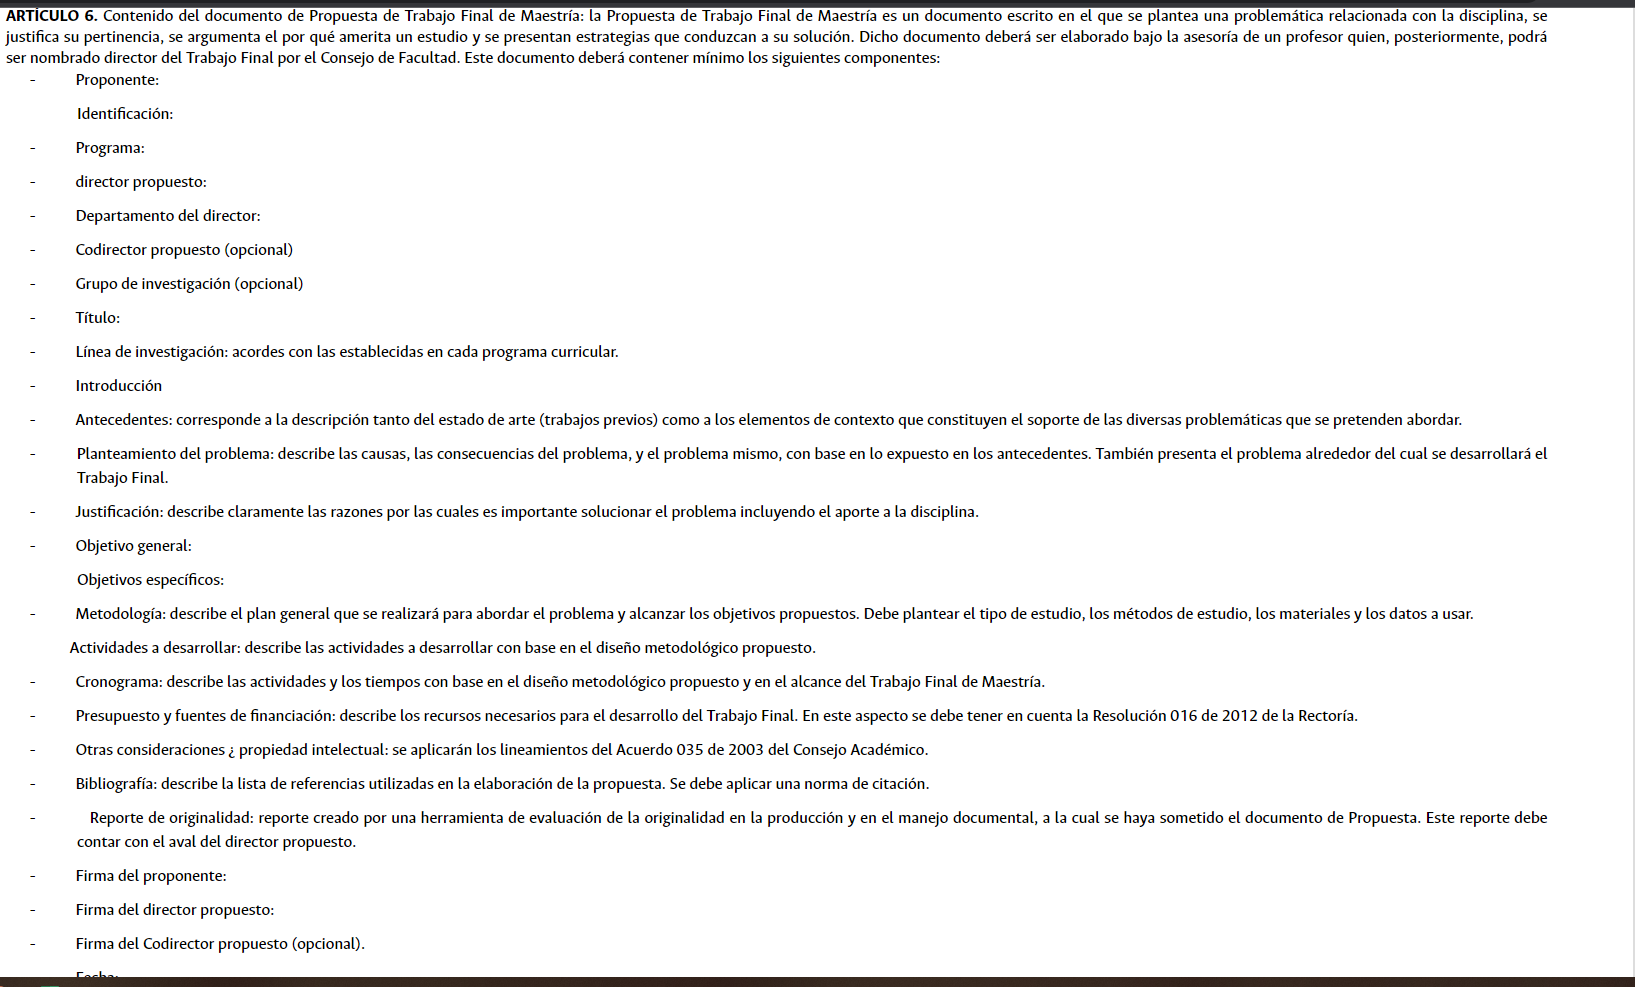
\includegraphics[width=0.8\textwidth]{propProf.png}
\end{frame}

\begin{frame}[c]{Esquema propuesta t\'esis de  maestr\'ia}
\href{http://www.legal.unal.edu.co/rlunal/home/doc.jsp?d_i=97946}{Acuerdo 104 2020, art\'iculo 20}
\centering
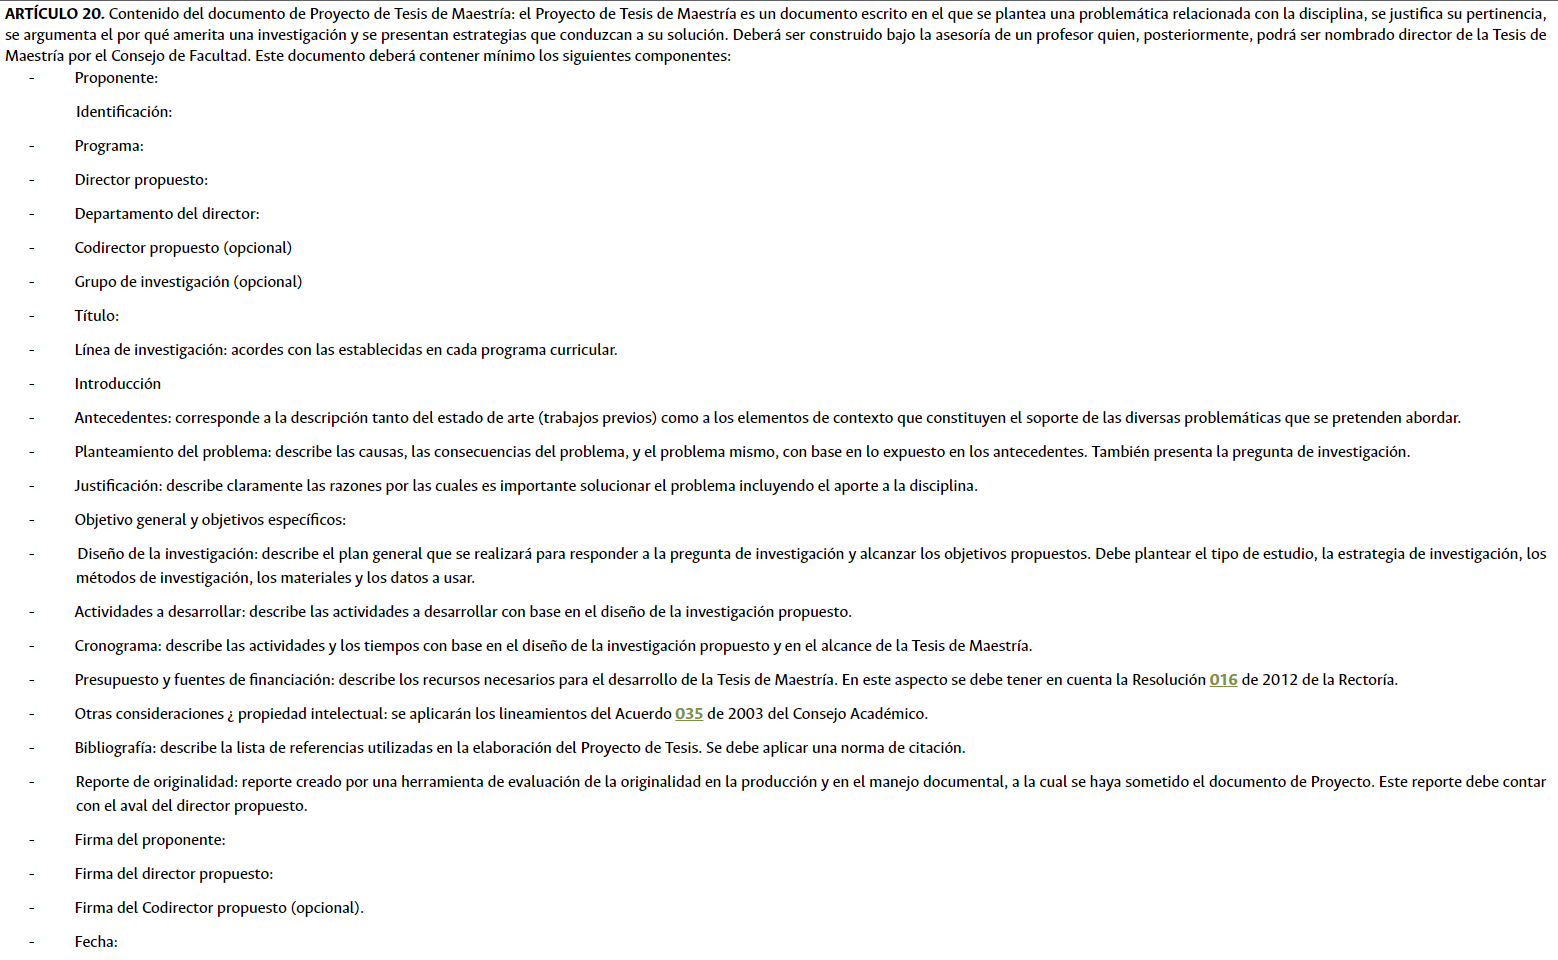
\includegraphics[width=0.8\textwidth]{propInve.png}
\end{frame}

\begin{frame}[c]{Plantillas}
\begin{itemize}
\item  \href{https://ingenieria.bogota.unal.edu.co/es/dependencias/vicedecanatura-academica/formatos.html}{Plantilla trabajo final de maestr\'ia}
\item  \url{https://ingenieria.bogota.unal.edu.co/es/dependencias/vicedecanatura-academica/formatos.html}
\item  \href{https://ingenieria.bogota.unal.edu.co/es/dependencias/vicedecanatura-academica/formatos.html}{Plantilla tesis de maestr\'ia}
\end{itemize}
\end{frame}


%---
\section{Planeaci\'on de la propuesta}
\begin{frame}[c]{Pasos para la planeaci\'on de la propuesta}
\begin{enumerate}
\item Determinar el argumento, pregunta de investigaci\'on o hipot\'esis.
\item Identificar revistas, autores, grupos de investigaci\'on claves en el tema de inter\'es.
\item Revisar bibliograf\'ia de los \'ultimos 4 a\~nos en principio. 
\item Leer con un propop\'osito. Leer mucho.
\item Organizar las notas de la revisi\'on bibliogr\'afica.
\item Escribir un primer borrador de la propuesta. 
\end{enumerate}
\end{frame}


\end{document}


